% This file was created by matlab2tikz.
%
%The latest updates can be retrieved from
%  http://www.mathworks.com/matlabcentral/fileexchange/22022-matlab2tikz-matlab2tikz
%where you can also make suggestions and rate matlab2tikz.
%
\definecolor{mycolor1}{rgb}{0.00000,0.44700,0.74100}%
%
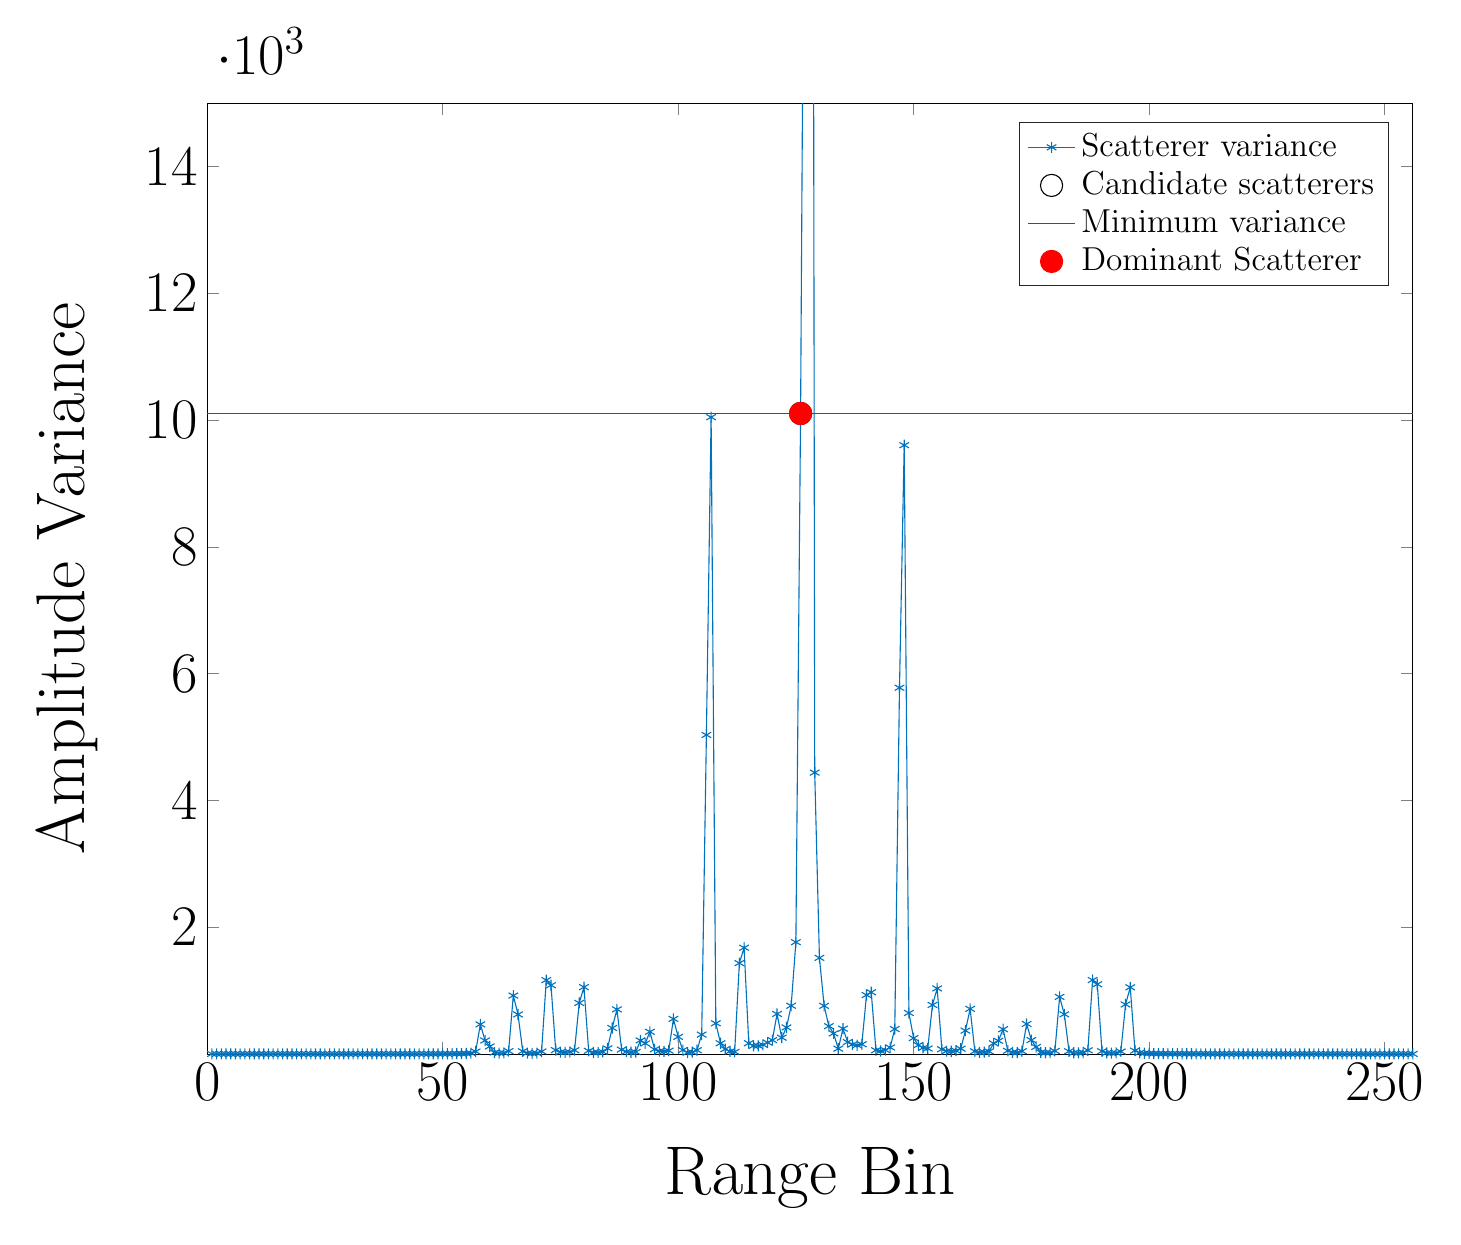
\begin{tikzpicture}

\begin{axis}[%
width=6.028in,
height=4.754in,
at={(1.011in,0.642in)},
scale only axis,
xmin=0,
xmax=256,
xlabel style={font=\fontsize{25}{20}\selectfont\color{black}, yshift = -10},
xlabel={Range Bin},
ymin=0,
ymax=1.5e4,
ylabel style={font=\fontsize{25}{20}\selectfont\color{black}, yshift=10pt},
ylabel={Amplitude Variance},
axis background/.style={fill=white},
tick label style={font=\fontsize{20}{11}\selectfont\color{black}},
xtick distance = 50,
ytick distance=2e3,
yticklabel={\ifdim\tick pt=0pt\else\pgfmathprintnumber{\tick}\fi}, 
scaled y ticks=base 10:-3,
legend style={legend cell align=left, align=left, draw=white!15!black, font=\fontsize{12}{11}\selectfont\color{black}}
]
\addplot [color=mycolor1, mark=asterisk, mark options={solid, mycolor1}]
  table[row sep=crcr]{%
1	2.08321120363209\\
2	1.921904220233\\
3	1.92674362838173\\
4	1.93310144062469\\
5	1.94669622820027\\
6	1.94115478170521\\
7	1.96152333731778\\
8	1.94910798661964\\
9	1.93293267162336\\
10	1.9370473039196\\
11	2.04531502880971\\
12	2.0606074290485\\
13	2.05879951018943\\
14	1.95354714810257\\
15	2.04713092781947\\
16	2.07259003245576\\
17	2.18431716078799\\
18	2.16139285444331\\
19	1.99396514031343\\
20	2.02973960572453\\
21	2.14614518580977\\
22	2.06806558423006\\
23	2.14220786459038\\
24	2.10473044070364\\
25	2.19948889686861\\
26	2.05653994475873\\
27	2.11939291246629\\
28	2.14611488050265\\
29	2.24321711627365\\
30	2.22880779286643\\
31	2.34071037680191\\
32	2.35206267420149\\
33	2.63461240823655\\
34	2.53076965136433\\
35	2.5465674475122\\
36	2.44144910314457\\
37	2.67448674994679\\
38	2.68415813541077\\
39	2.71117842178543\\
40	2.79559045507104\\
41	2.72976214134926\\
42	2.9639386978755\\
43	2.9310724812868\\
44	2.98099508162445\\
45	3.17148203971716\\
46	3.34720133263892\\
47	3.44439859826344\\
48	3.61635200102043\\
49	3.7759460725445\\
50	4.24222884610444\\
51	4.41171653170368\\
52	4.86593602438878\\
53	5.59652722717545\\
54	6.83990514628735\\
55	8.7606167327905\\
56	15.1603291346533\\
57	39.857714591742\\
58	468.414312043591\\
59	214.15175500521\\
60	120.440382079514\\
61	23.8930464799152\\
62	15.3780020307775\\
63	18.8290993610706\\
64	46.6595174702634\\
65	922.568143445766\\
66	625.032365962269\\
67	44.05704330227\\
68	15.8644269339805\\
69	11.1725332061883\\
70	14.774710426899\\
71	40.5568358714716\\
72	1166.51692115366\\
73	1085.9702957141\\
74	62.0786532552127\\
75	30.9275788643156\\
76	26.7034698019049\\
77	32.6570858563442\\
78	60.6024460813725\\
79	806.370147932657\\
80	1055.5193335565\\
81	51.2091939438542\\
82	24.8237285196772\\
83	25.1471914630608\\
84	35.0129877460332\\
85	89.9765017262348\\
86	411.117168196505\\
87	704.521170856365\\
88	69.8777390161609\\
89	37.0737945028782\\
90	28.5321859248087\\
91	31.9567938559395\\
92	214.738533972753\\
93	167.318855751845\\
94	351.194143609148\\
95	74.2033347684922\\
96	47.1964462660784\\
97	41.1179678766444\\
98	53.9346322088505\\
99	555.235116840062\\
100	271.105771199784\\
101	62.8204179279888\\
102	23.7060761281031\\
103	29.1567725004453\\
104	60.8001855915124\\
105	307.0127762513\\
106	5034.48602161453\\
107	10047.2654511405\\
108	485.507187625322\\
109	170.32593734737\\
110	77.8493602408992\\
111	42.1948403667143\\
112	34.543033491961\\
113	1434.85050890689\\
114	1677.30095682208\\
115	171.046746001318\\
116	129.608089351639\\
117	130.119737254404\\
118	146.254578180326\\
119	181.054746006636\\
120	219.673286895483\\
121	632.649378056554\\
122	258.319822006803\\
123	419.48237887866\\
124	762.206044343748\\
125	1765.17471336436\\
126	10105.9322692203\\
127	22343.0539690425\\
128	52002.0409624597\\
129	4440.50813594317\\
130	1517.72141953784\\
131	760.764860530975\\
132	439.952566550395\\
133	325.073950651625\\
134	84.8916248026265\\
135	401.030102879254\\
136	188.4339020801\\
137	151.291225738727\\
138	138.967998223346\\
139	154.532662152589\\
140	931.236137173979\\
141	974.693206409318\\
142	60.0389147242318\\
143	48.0782970824718\\
144	62.4614636684976\\
145	103.841355927459\\
146	394.625533895844\\
147	5778.93574663015\\
148	9605.30431010017\\
149	647.922368646472\\
150	251.903487235542\\
151	141.207447634804\\
152	98.4228440450755\\
153	87.2835365460573\\
154	774.741761291363\\
155	1035.16198124819\\
156	75.0949669730951\\
157	47.1659715713286\\
158	43.9615843216195\\
159	52.9246787795588\\
160	85.1766827907494\\
161	369.370655894115\\
162	712.832183815632\\
163	43.6009739684981\\
164	27.8774282565255\\
165	30.7438787833207\\
166	41.6640871276399\\
167	169.245363794576\\
168	208.886236902711\\
169	391.750397461381\\
170	51.884188748898\\
171	26.9271548887131\\
172	23.77651623404\\
173	44.8021266942446\\
174	475.191624895443\\
175	220.283677369054\\
176	111.704438402747\\
177	27.1069952933976\\
178	20.1970746318427\\
179	21.6880541826496\\
180	49.2016026434613\\
181	901.98008777202\\
182	626.601268010464\\
183	44.1751687210038\\
184	20.2924146303747\\
185	17.4698168063274\\
186	24.5808853810647\\
187	58.9598628629286\\
188	1167.94979218178\\
189	1101.1811446464\\
190	44.5268793670615\\
191	17.9525560171142\\
192	14.4164991884608\\
193	18.7429427213321\\
194	39.8908113734624\\
195	782.795027117167\\
196	1053.17281965714\\
197	54.4759865138814\\
198	21.023955173951\\
199	12.463373161777\\
200	9.46280492938718\\
201	7.56221499198981\\
202	6.73711559281714\\
203	6.30383970438473\\
204	5.91551964608533\\
205	5.63258441170031\\
206	5.21877238604558\\
207	5.03659259613409\\
208	4.80044923921998\\
209	4.36802497130052\\
210	4.15476409241554\\
211	4.17955811497718\\
212	4.06456431004751\\
213	3.88415712535343\\
214	3.47659324750515\\
215	3.50194995122602\\
216	3.41268553750496\\
217	3.29023866229171\\
218	3.19060276195639\\
219	2.93870295146985\\
220	2.95272004449474\\
221	2.90255975777407\\
222	2.74807661107966\\
223	2.52835561147921\\
224	2.59918542173538\\
225	2.57146911719801\\
226	2.53875574874579\\
227	2.53371037121738\\
228	2.46559630817839\\
229	2.40884871847049\\
230	2.33789960933137\\
231	2.35200337423874\\
232	2.38004200076115\\
233	2.28926007940636\\
234	2.4326449579174\\
235	2.17387728846157\\
236	2.23416275002014\\
237	2.27313892893194\\
238	2.23653480673665\\
239	2.11207522728423\\
240	2.15124355169376\\
241	2.16217914832361\\
242	2.19569842630966\\
243	2.01961128525521\\
244	1.97298210453101\\
245	2.04204682136496\\
246	1.96305099932611\\
247	1.97122502172868\\
248	2.03333164065216\\
249	1.93804657326272\\
250	2.00670065443835\\
251	2.0374039342196\\
252	1.98702064338366\\
253	1.91936262117433\\
254	1.98105547011769\\
255	1.83687871903398\\
256	1.91547878858092\\
};
\addlegendentry{Scatterer variance}

\addplot [color=black, only marks, mark size=4.0pt, mark=o, mark options={solid, black}]
  table[row sep=crcr]{%
126	10105.9322692203\\
127	22343.0539690425\\
128	52002.0409624597\\
};
\addlegendentry{Candidate scatterers}

\addplot [color=red]
  table[row sep=crcr]{%
0	10105.9322692203\\
300	10105.9322692203\\
};
\addlegendentry{Minimum variance}

\addplot [color=red, only marks, mark size=4.0pt, mark=*, mark options={solid, fill=red, red}]
  table[row sep=crcr]{%
126	10105.9322692203\\
};
\addlegendentry{Dominant Scatterer}

\end{axis}
\end{tikzpicture}%